
\section{Supervised Learning and Generalization}
\label{ex:1}


\setcounter{subsection}{2}
\subsection{In the Wide Jungle of the Training}
\label{ex:1.3}


\begin{task}{1.3.1}
  % What is the impact of the noise (parameter \texttt{noise} in the notebook) with respect to the
  % optimization process?
\end{task}

The noise parameter controls the deviation of the training data from the true function.
Figure~\ref{fig:ex1_noise-level} shows the impact of noise on the optimization process. For $noise =
  0$, the data exactly matches the true function and the model will converge to the true function
quickly. For $noise > 0$, the data is perturbed by noise and the model will take longer to converge.
For $noise = 1$, the data is completely random and the model will only converge to the mean of the
training data without being able to capture the underlying function.


\begin{task}{1.3.2}
  % How does (vanilla) gradient descent compare with respect to its stochastic and accelerated
  % versions?
\end{task}

Vanilla gradient descent is the slowest of the three methods. It computes the gradient of the loss
function for the entire training set at each iteration. Stochastic gradient descent (SGD) is faster
than vanilla gradient descent, because it computes the gradient for a random subset of the training
data at each iteration. However it has a higher variance in the loss function. Accelerated gradient
descent is the fastest of the three methods. It uses a momentum term to speed up convergence and
reduce oscillations in the loss function.


\begin{task}{1.3.3}
  % How does the size of the network impact the choice of the optimizer?
\end{task}

For small networks, vanilla gradient descent is sufficient, because the computation of the gradient
is not very expensive. For larger networks, SGD is more appropriate due to its lower computational
cost. Accelerated gradient descent is the best choice for very large networks, because it converges
faster than the other two methods.


\begin{task}{1.3.4}
  % Discuss the difference between epochs and time to assess the speed of the algorithms. What can it
  % mean to converge fast?
\end{task}

The model is trained for $2500$ epochs. In Figure~\ref{fig:ex1_optimizers}, we can see that SGD with
a learning rate of $0.05$ and without momentum has an average training time, but very slow
convergence. Using a learning rate of $0.1$ already converges much faster, but also takes longer to
compute. Momentum has a similar convergence rate and is much quicker to compute, but also has high
variance. The Adam and the LBFGS optimizers converge the fastest, but LBFGS has the longest
computational time. The Adam optimizer is the best choice for this problem, because it converges
quickly and has low variance. All optimizers except for vanilla SGD with learning rate $0.05$ can
be considered to have converged after at most $1000$ epochs.

\begin{figure}[ht!]
  \centering
  \begin{minipage}{0.48\textwidth}
    \centering
    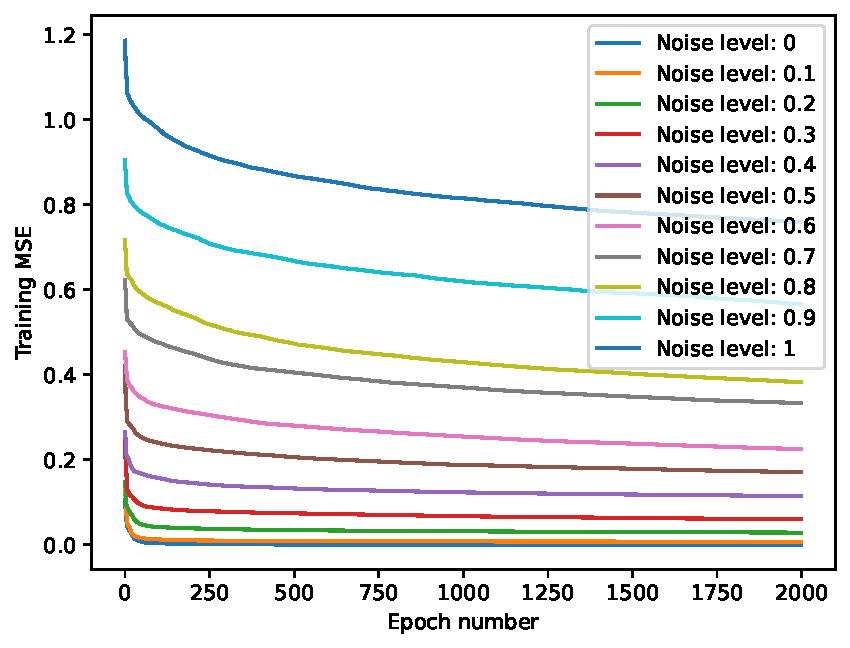
\includegraphics[width=0.9\linewidth]{ex1_noise-level.pdf}
    \captionof{figure}{Impact of noise on the optimization process}
    \label{fig:ex1_noise-level}
  \end{minipage}
  \begin{minipage}{0.48\textwidth}
    \centering
    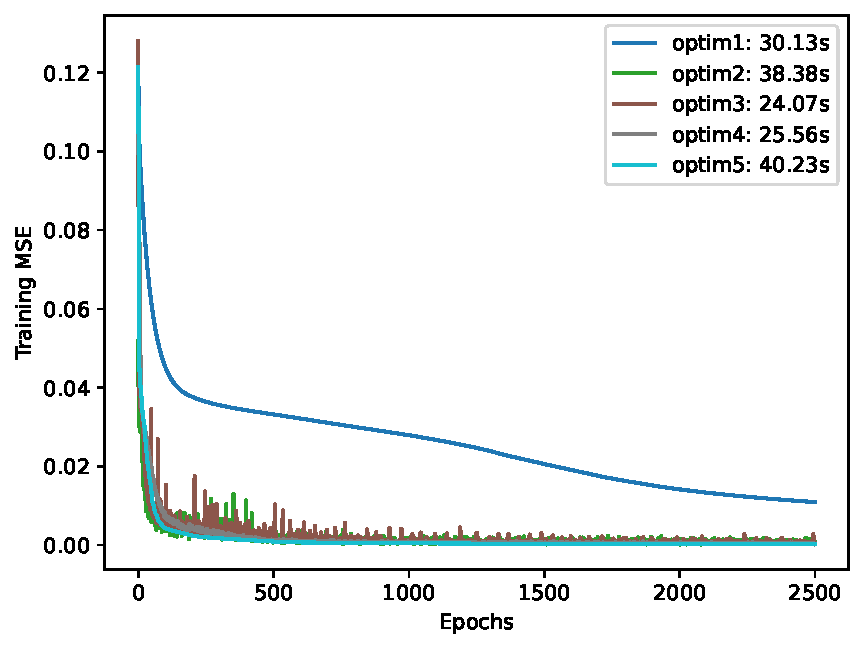
\includegraphics[width=0.9\linewidth]{ex1_optimizers.pdf}
    \captionof{figure}{Comparison of optimizers}
    \label{fig:ex1_optimizers}
  \end{minipage}
\end{figure}


\subsubsection*{A bigger model}
\begin{task}{1.3.5}
  % How many parameters does the model have?
\end{task}

The model has $34826$ parameters in total as shown in Table~\ref{tab:ex1_model}.

\begin{table}[ht!]
  \begin{tabular}{|l|l|r|}
    \hline
    \textbf{Layer Type} & \textbf{Shape} & \textbf{\# Param} \\ \hline
    (Input)             & (28, 28, 1)    & 0                 \\ \hline
    Conv2D              & (26, 26, 32)   & 320               \\ \hline
    MaxPooling2D        & (13, 13, 32)   & 0                 \\ \hline
    Conv2D              & (11, 11, 64)   & 18496             \\ \hline
    MaxPooling2D        & (5, 5, 64)     & 0                 \\ \hline
    Flatten             & (1600, )       & 0                 \\ \hline
    Dropout             & (1600, )       & 0                 \\ \hline
    Dense               & (10, )         & 16010             \\ \hline\hline
    \textbf{Total}      &                & \textbf{34826}    \\ \hline
  \end{tabular}
  \centering
  \caption{Model parameters}
  \label{tab:ex1_model}
\end{table}


\begin{task}{1.3.6}
  % Replace the ADAM optimizer by a SGD one. Can you still achieve excellent performances? Try then
  % the Adadelta optimizer. What is its particularity?
\end{task}

The SGD optimizer has a much slower convergence rate than the Adam optimizer as shown in
Figure~\ref{fig:ex1_mnist_optimizers}. The Adadelta optimizer achieves very good performance after
the first epoch already and has a low variance. The Adam optimizer is in between the two in
terms of convergence rate and variance. Compared to the Adam optimizer, the Adadelta optimizer
does not require a learning rate to be set, because it uses the gradient and the average of
the squared gradient over a window of time steps to adapt the learning rate.



\subsection{A Personal Regression Exercise}
\label{ex:1.4}

\begin{task}{1.4.1}
  % Define your training and testing dataset using respectively 2000 and 1000 samples drawn
  % independently. Explain the point of having different datasets for training and testing. Plot the
  % surface associated to the training set.
\end{task}

\begin{figure}[ht!]
  \centering
  \begin{minipage}{0.48\textwidth}
    \centering
    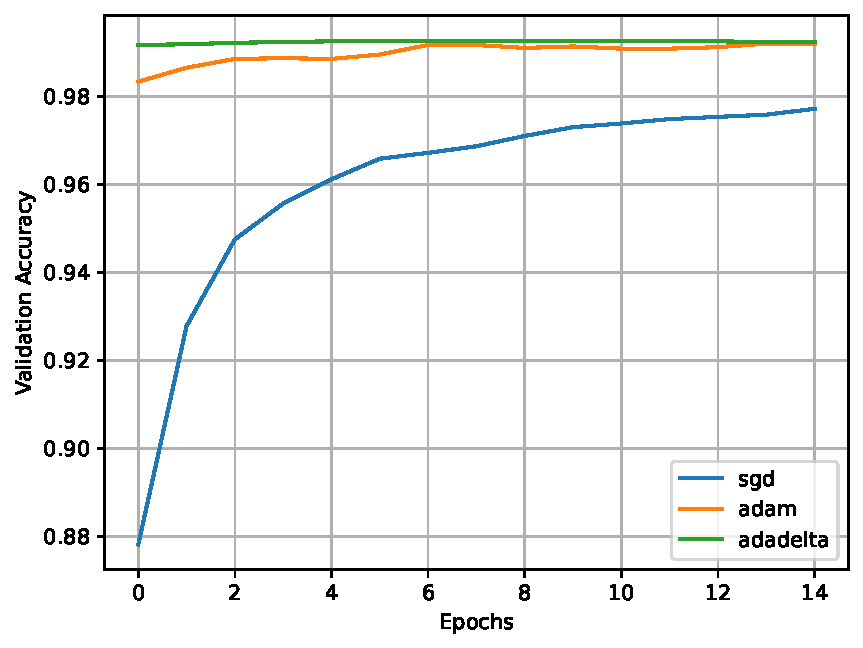
\includegraphics[width=0.9\linewidth]{ex1_mnist_optimizers.pdf}
    \captionof{figure}{Validation accuracy}
    \label{fig:ex1_mnist_optimizers}
  \end{minipage}
  \begin{minipage}{0.48\textwidth}
    \centering
    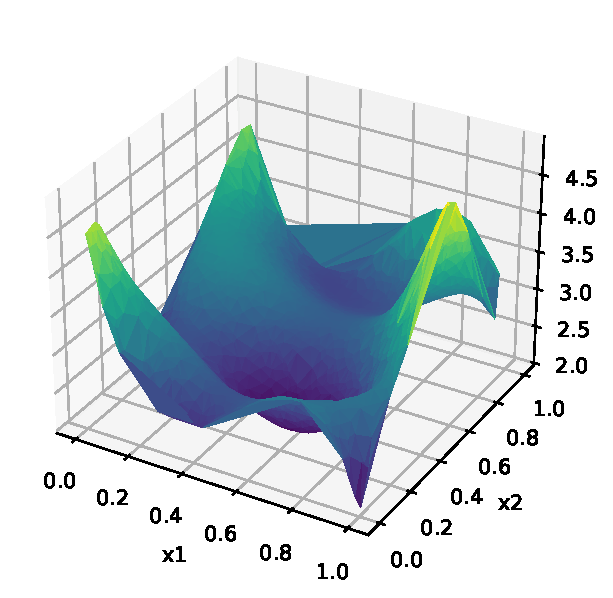
\includegraphics[width=0.9\linewidth]{ex1_regression_train.pdf}
    \captionof{figure}{Function surface of the training data}
    \label{fig:ex1_regression_train}
  \end{minipage}
\end{figure}

If the same dataset is used for training and testing, the model will overfit the data and not
generalize well to unseen data. Moreover, the evaluation of the model will be biased, because the
model has already seen the test data during training. If two independent datasets are used, the
performance on the test data corresponds more to real-world performance, where the model has not
seen the data before. Also, the performance on the test data will be bad, if the model has overfit
the training data. The surface associated to the training set is shown in
Figure~\ref{fig:ex1_regression_train}.


\begin{task}{1.4.2}
  % Build and train your feedforward neural network. To that end, you must perform an adequate model
  % selection on the training set. Investigate carefully the architecture of your model: number of
  % layers, number of neurons, learning algorithm and transfer function. How do you validate your
  % model?
\end{task}

The model architecture is shown in Table~\ref{tab:ex1_regression_model}. The choice of the
activation functions seemed to have the biggest impact on the performance. The \texttt{mish}
activation function performed much better than the other functions I tried. Increasing the number of
layers and neurons also improved the performance. However, the model was overfitting the training
data when using too many neurons. The choice of the optimizer and the learning rate did not have a
big impact on the performance. Here, I used the Adam optimizer with a learning rate of $0.05$. All
choices were validated by calculating the mean squared error on the test data.

\begin{table}[ht!]
  \centering
  \begin{tabular}{|l|l|l|r|}
    \hline
    \textbf{Layer Type} & \textbf{Shape} & \textbf{Activation Function} & \textbf{\# Param} \\ \hline
    Dense               & (16)           & mish                         & 48                \\ \hline
    Dense               & (16)           & mish                         & 272               \\ \hline
    Dense               & (16)           & tanh                         & 272               \\ \hline
    Dense               & (1)            & (None)                       & 17                \\ \hline\hline
    \textbf{Total}      &                &                              & \textbf{609}      \\ \hline
  \end{tabular}
  \caption{Regression model parameters}
  \label{tab:ex1_regression_model}
\end{table}


\begin{task}{1.4.3}
  % Evaluate the performance of your selected network on the test set. Plot the surface of the test
  % set and the approximation given by the network. Explain why you cannot train further. Give the
  % final MSE on the test set.
\end{task}

The surfaces of the test data and the predicted data are shown in
Figure~\ref{fig:ex1_regression_surface}. The model has already converged and further training would
not improve the performance. The final mean squared error on the test data is $0.0017132$.

\begin{figure}[ht!]
  \centering
  \begin{subfigure}{0.49\textwidth}
    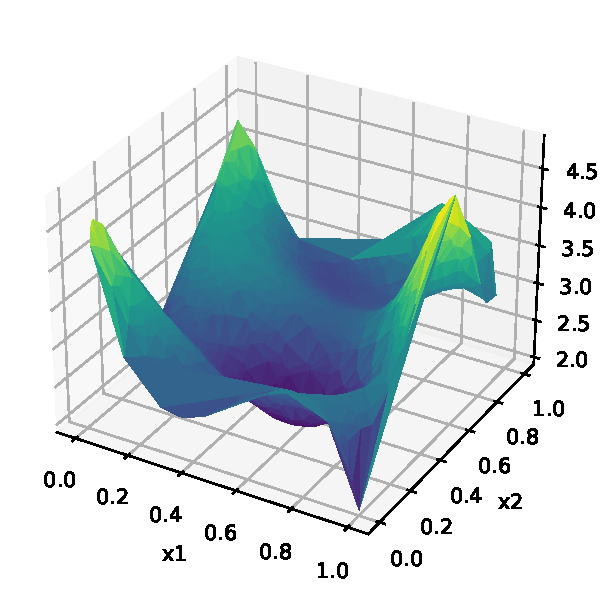
\includegraphics[width=\textwidth]{ex1_regression_test.pdf}
    \caption{Test data}
    \label{fig:ex1_regression_test}
  \end{subfigure}
  \begin{subfigure}{0.49\textwidth}
    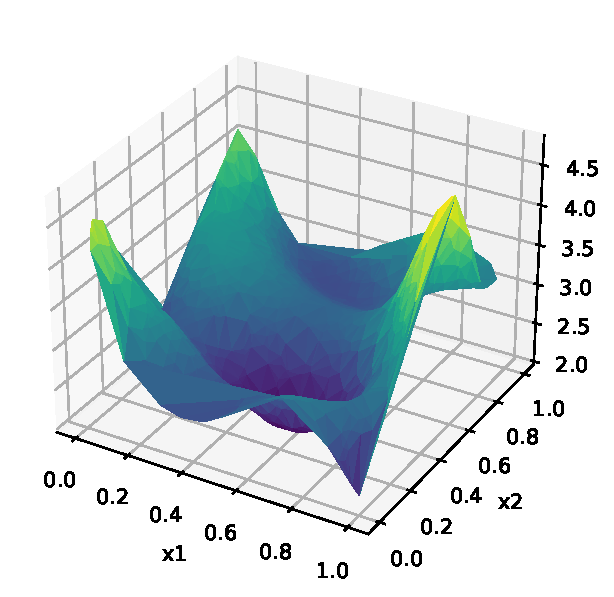
\includegraphics[width=\textwidth]{ex1_regression_predicted.pdf}
    \caption{Predicted}
    \label{fig:ex1_regression_predicted}
  \end{subfigure}
  \caption{Function surface}
  \label{fig:ex1_regression_surface}
\end{figure}


\begin{task}{1.4.4}
  % Describe the regularization strategy that you used to avoid overfitting. What other strategy can you
  % think of?
\end{task}

I used early stopping to avoid overfitting. The training was stopped when the validation loss did
not improve for $10$ epochs. Another strategy to avoid overfitting is to use dropout layers, which
sets a few neurons to zero during training.
